\begin{frame}
\frametitle{Komparator}
\framesubtitle{}
    \begin{block}{Komparator}
        \begin{itemize}
            \item OPV vergleicht die Eingangspannungen $U_{in}$ und $U_{ref}$
            am invertierenden bzw nichtinvertierden Eingang.   
            \item $U_{in} > U_{ref}$: OPV gibt die an $V^+ (7)$ angelegte
            Spannung aus, andernfalls $V^- (4)$.
        \end{itemize}
    \end{block}
    \begin{block}{Technische Funktionsweise:}
        \begin{itemize}
            \item Differenzverstärker verstärkt $U_{in} - U_{out}$
            \item zusätzlicher Verstärker $\rightarrow$ $U_{out}$ erreicht sehr schnell die maximal mögliche
            Verstärkung (=Versorgungsspannung)
        \end{itemize}
    \end{block}
\end{frame}

\begin{frame}
\frametitle{Versuchsaufbau}
\framesubtitle{}
    \begin{block}{Aufbau}
         \begin{itemize}
             \item Komperator wurde ohne Last am Ausgang mit Spannung $\pm 9V$
             betrieben
             \item $U_{in}$ wurde in Abhängigkeit von $U_{ref}$ untersucht
             \item besonder von Interesse: Umschaltpunkt
         \end{itemize}
    \end{block}
    \begin{figure}[H]
    \begin{center}
            \includegraphics[scale=0.2]{./img/schaltung/komparator_1.png}
    \end{center}
    \end{figure}
\end{frame}

\begin{frame}
\frametitle{}
\framesubtitle{}
    \begin{columns}[c]

    \column{0.5\textwidth}
    \begin{figure}[H]
    \begin{center}
            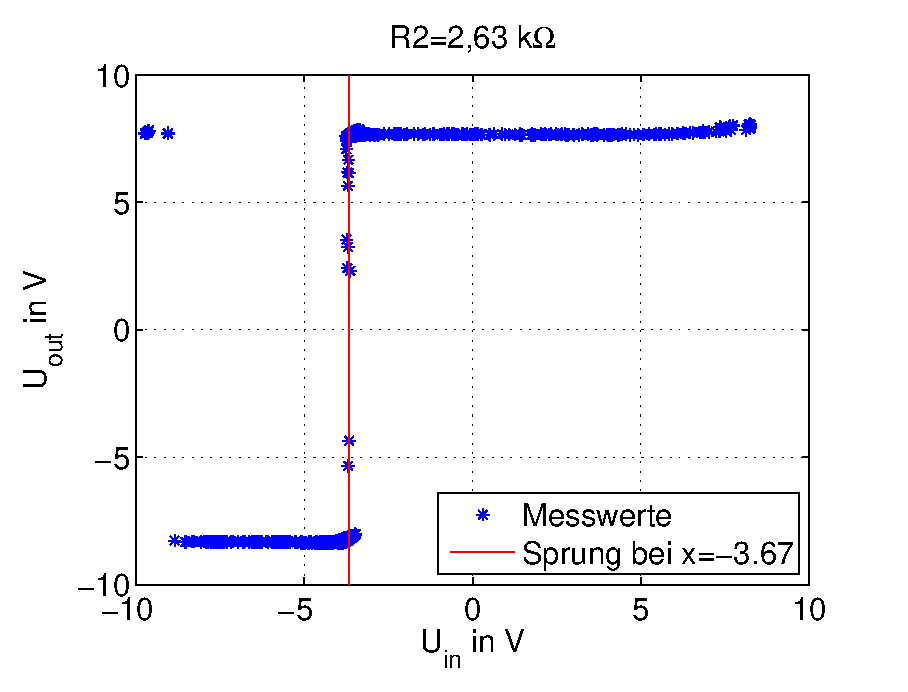
\includegraphics[scale=0.32]{./img/plots/Auf_1_2_63_Ohm.eps}
    \end{center}
    \end{figure}
    \begin{figure}[H]
    \begin{center}
            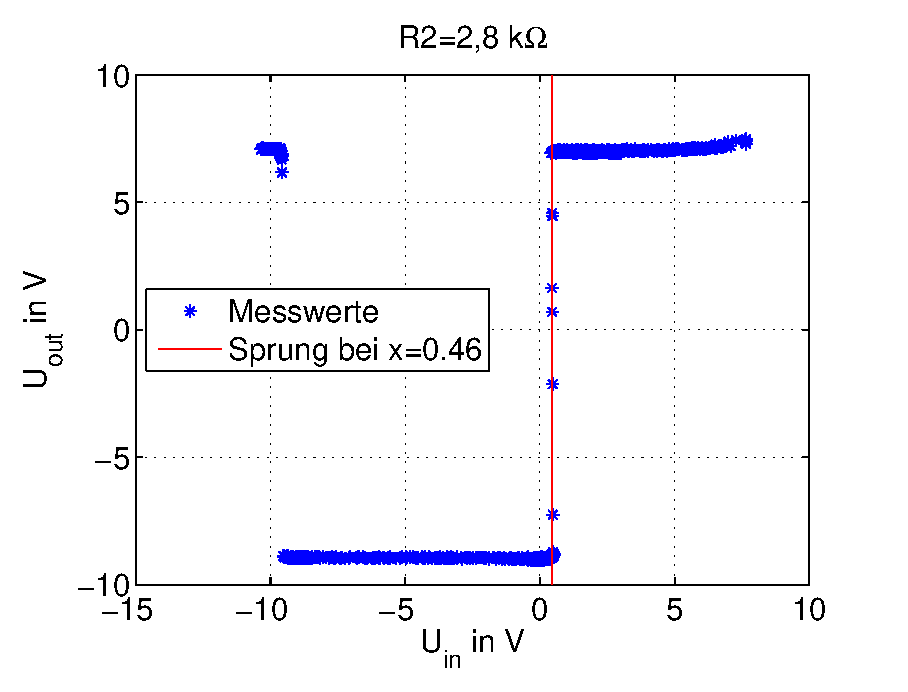
\includegraphics[scale=0.32]{./img/plots/Auf_1_2_8_Ohm_1.eps}
    \end{center}
    \end{figure}
    \column{0.5\textwidth}
    \begin{figure}[H]
    \begin{center}
            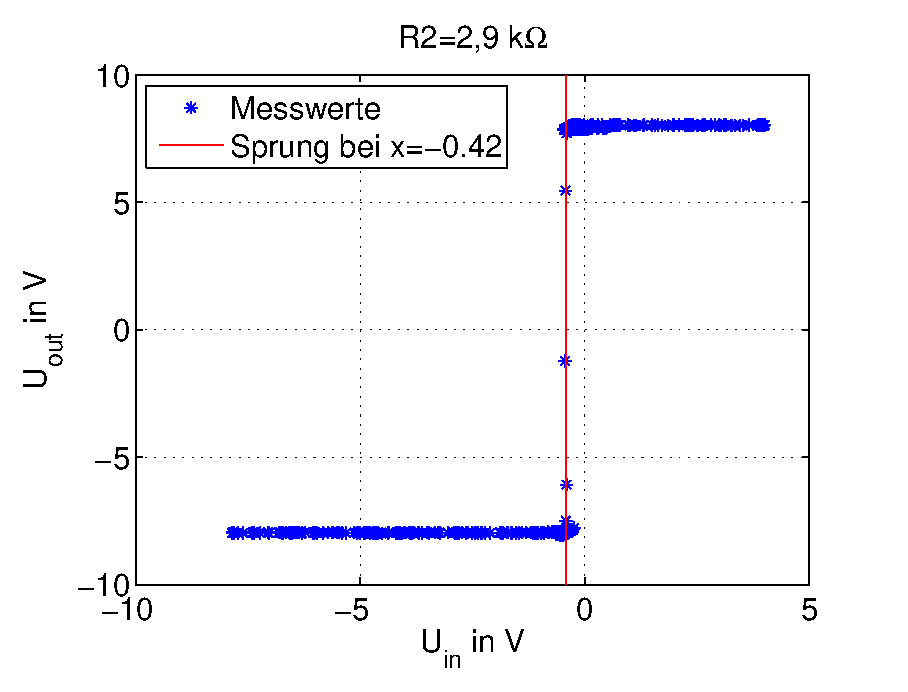
\includegraphics[scale=0.32]{./img/plots/Auf_1_2_9_Ohm.eps}
    \end{center}
    \end{figure}
    \begin{figure}[H]
    \begin{center}
            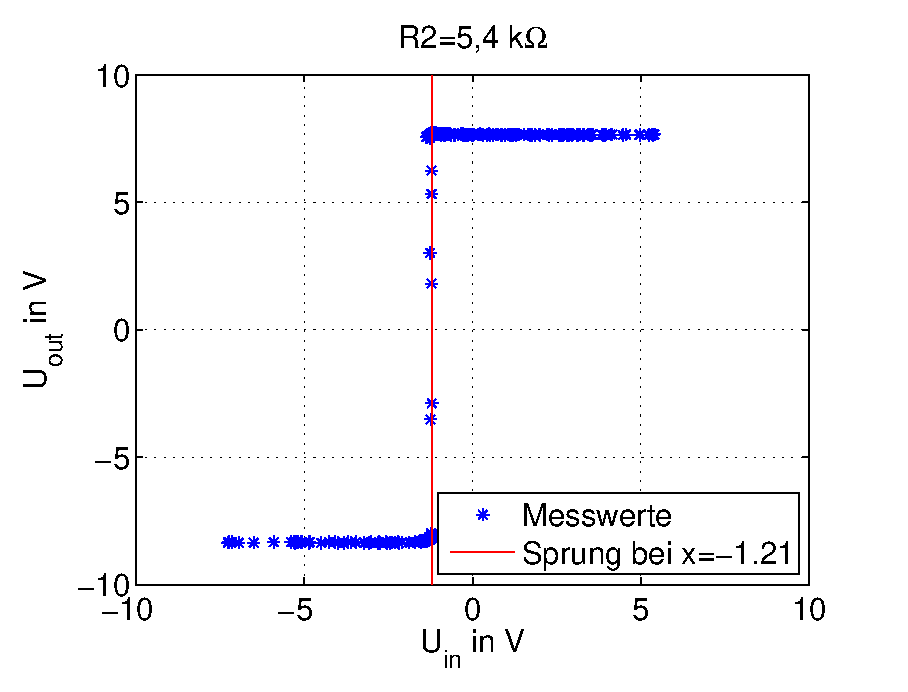
\includegraphics[scale=0.32]{./img/plots/Auf_1_5_4_Ohm.eps}
    \end{center}
    \end{figure}
        
    \end{columns}
\end{frame}

\begin{frame}
\frametitle{Ergebnisse}
\framesubtitle{} 
    %\begin{columns}[c]
    %    \column{0.5\textwidth}
    %    \column{0.5\textwidth}
    %    %\begin{tabular}{c||c|c}
    %    %     $R$ & $U_{ref}$ aus $R$ & Sprungwert \\
    %    %    \hline
    %    %    $2.63\Omega$& $V$& $-3.67V$  \\
    %    %    $2.9\Omega$& $V$& $-0.42V$  \\
    %    %    $2.8\Omega$& $V$& $0.46V$  \\
    %    %    $5.4\Omega$& $V$& $-1.21V$  
    %    %\end{tabular}
    %\end{columns}
    \begin{block}{Auswertung}
        \begin{itemize}
            \item Ergebnisse stimmen i.A gut mit Theorie überein
            \item $U_{out}$ liegt nicht ganz bei $\pm 9V$ $\rightarrow$ Bauart
            des Komparators limitiert $V_{out}$
            \item Verstärkungsfaktor (gemittelt): $V$
        \end{itemize}
    \end{block}
\end{frame}

\begin{frame}
\frametitle{Auffälligkeiten}
\framesubtitle{}
    \begin{columns}[c]
        \column{0.6\textwidth}     
            \begin{block}{negativer Sprung}
                 \begin{itemize}
                     \item weiterer Sprung bei $U_{in} = -9.83V$
                 \end{itemize}
            \end{block}
        \column{0.6\textwidth}     
            \begin{figure}[H]
            \begin{center}
                    \includegraphics[scale=0.3]{./img/plots/Auf_1_2_8_Ohm_2.eps}
            \end{center}
            \end{figure}
    \end{columns}
\end{frame}
\begin{frame}
\frametitle{Auffälligkeiten}
\framesubtitle{}
    \begin{columns}[c]
        \column{0.6\textwidth}     
            \begin{block}{negativer Sprung}
                 \begin{itemize}
                     \item weiterer Sprung bei $U_{in} = -9.83V$
                 \end{itemize}
            \end{block}
            \begin{block}{Messungenauigkeit}
                 \begin{itemize}
                     \item Sehr ungenaue Messung im Sprungbereich
                     \item Überlagerung der $x$-Werte macht Fitten schwierig
                     \item "An Schieber regeln" ist keine gute Messmethode
                 \end{itemize}
            \end{block}
        \column{0.6\textwidth}     
            \begin{figure}[H]
            \begin{center}
                    \includegraphics[scale=0.3]{./img/plots/Auf_1_2_8_Ohm_2.eps}
            \end{center}
            \end{figure}
            \begin{figure}[H]
            \begin{center}
                    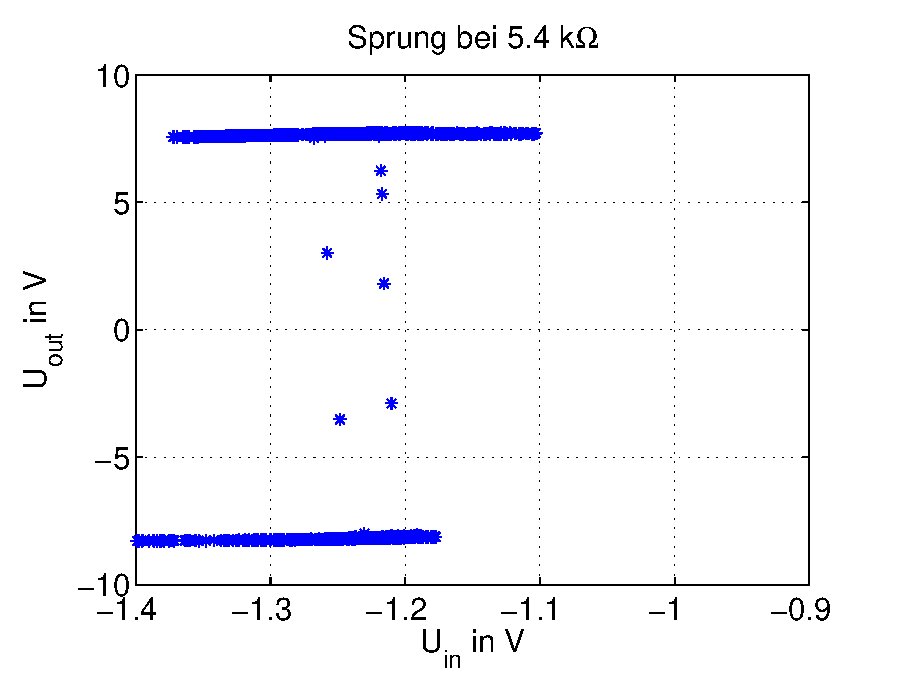
\includegraphics[scale=0.3]{./img/plots/Auf_1_5_4_Sprung.eps}
            \end{center}
            \end{figure}
            
    \end{columns}
\end{frame}

\begin{frame}
\frametitle{Versuchsaufbau mit LED}
\framesubtitle{}
    \begin{block}{Aufbau}
         \begin{itemize}
             \item LED mit Last (zum Schutz der LED) wurde eingebaut
             \item Betrieb mit sinusförmiger Wechselspannung
             \item Untersuchung des Verhaltens am Oszilloskop
         \end{itemize}
    \end{block}
    \begin{figure}[H]
    \begin{center}
            \includegraphics[scale=0.2]{./img/schaltung/komparator_2.png}
    \end{center}
    \end{figure}
\end{frame}
\begin{frame}
\frametitle{Ergebnis}
\framesubtitle{}
    \begin{columns}[c]
    \column{0.6\textwidth}
    \begin{block}{Betrachtung}
        \begin{itemize}
            \item Komparator erzeugt verstärkte Rechteckspannung 
            \item Komperator "schaltet" wenn $U_{in} > U_{ref}$
            \item $Amplitude(U_{out}) < 18V$
            \item LED blinkt regelmäßig
        \end{itemize}
    \end{block}
    \begin{block}{Erklärung:}
        \begin{itemize}
            \item Verhalten erkärt sich direkt aus vorherigen Ergebnissen
            \item Komparator kann Rechtecksspannung erzeugen $\rightarrow$
            Verwendung für Blinkschaltung
        \end{itemize}
    \end{block}
    \column{0.6\textwidth}
    \begin{figure}[H]
    \begin{center}
            \includegraphics[scale=0.15]{./img/oszi/scope_1.png}
    \end{center}
    \begin{description}
        \item[Gelb]: $U_{in}$
        \item[Rosa]: $U_{ref}$
        \item[Grün]: $U_{out}$
    \end{description}
    \end{figure}
    \end{columns}
\end{frame}
